\documentclass{article}
\usepackage[utf8]{inputenc}
\usepackage[a4paper, top=2cm, bottom=2cm, left=2cm, right=2cm]{geometry}
\usepackage{amsfonts}
\usepackage{amsmath}
\usepackage{amssymb}
\usepackage{amsthm}
\usepackage{esint}
\usepackage{fancyhdr}
\usepackage{enumitem}
\usepackage{amsmath}
\usepackage{amsthm}
\usepackage{amssymb}
\usepackage{mathabx}
\usepackage[linesnumbered , ruled , vlined]{algorithm2e}
\usepackage{listings}
\usepackage{xcolor}
\usepackage{floatrow}
\usepackage{graphicx}
\usepackage{fancyhdr}
\usepackage{listings}
\usepackage[hypcap=false]{caption}
\usepackage{hyperref}
\usepackage{subfig}
\usepackage{tikz}
\usepackage{hyperref}

\pagestyle{fancy}
\fancyhf{}
\lhead{200050107, 200050130, 200050154, 200050157}
\rhead{CS337}
\cfoot{\thepage}

\newcommand{\B}[1]{\textbf{#1}}
\newcommand{\I}[1]{\textit{#1}}

\title{\textbf{CS337 Course Project \\ Face Recognition}}
\author{Pranjal Kushwaha, Shashwat Garg, Vedang Asgaonkar, Virendra Kabra}
\date{Autumn 2022}

\begin{document}
\begin{sloppypar}       % for overfull, etc.

    \maketitle
    \tableofcontents

    \newpage

    \section{Dataset}
    
        \begin{itemize}
            \item We use the Labelled Faces in the Wild (LFW) dataset. It has been taken from \href{https://www.kaggle.com/datasets/jessicali9530/lfw-dataset}{Kaggle}. There is an uneven distribution of images, with only 10 people having at least 53 images. Thus, we train the model to classify these 10 people, with our dataset containing 53 images for each.
            \item The train-test split is 80-20, and the train set is further split to create the validation set. Equal splits are created for each class.
            \item \B{Data Augmentation}: We add horizontally flipped images to the dataset. This acts as a regularizer, helping the model to generalize better.
        \end{itemize}
    

    \section{Model Architecture}

        We use a Convolutional Neural Network (CNN) to create a multi-class image classifier. The network is inspired from FaceNet \cite{facenet}.

        \begin{center}
            \begin{table}[!h]
                \begin{tabular}{|c|c|c|c|c|}
                    \hline
                    \B{Layer} & \B{In} & \B{Out} & \B{Kernel} & \B{Params}\\
                    \hline \hline
                    conv1 & $250\times 250\times 3$ & $123\times 123\times 64$ & $7\times 7\times 3, 2$ & 9K\\
                    batchnorm1 & $123\times 123\times 64$ & $123\times 123\times 64$ & & 128\\
                    relu1 & $123\times 123\times 64$ & $123\times 123\times 64$ & & 0\\
                    maxpool1 & $123\times 123\times 64$ & $61\times 61\times 64$ & $2\times 2\times 64, 2$ & 0\\
                    dropout1 & $61\times 61\times 64$ & $61\times 61\times 64$ & & 0\\
                    \hline
                    conv2 & $61\times 61\times 64$ & $61\times 61\times 128$ & $3\times 3\times 64, 1$ & 74K\\
                    batchnorm2 & $61\times 61\times 128$ & $61\times 61\times 128$ & & 256\\
                    relu2 & $61\times 61\times 128$ & $61\times 61\times 128$ & & 0\\
                    maxpool2 & $61\times 61\times 128$ & $30\times 30\times 128$ & $2\times 2\times 128, 2$ & 0\\
                    dropout2 & $30\times 30\times 128$ & $30\times 30\times 128$ & & 0\\
                    \hline
                    conv3 & $30\times 30\times 128$ & $30\times 30\times 256$ & $3\times 3\times 128, 1$ & 295K\\
                    batchnorm3 & $30\times 30\times 256$ & $30\times 30\times 256$ & & 512\\
                    relu3 & $30\times 30\times 256$ & $30\times 30\times 256$ & & 0\\
                    maxpool3 & $30\times 30\times 256$ & $15\times 15\times 256$ & $2\times 2\times 128, 2$ & 0\\
                    dropout3 & $15\times 15\times 256$ & $15\times 15\times 256$ & & 0\\
                    \hline
                    conv4 & $15\times 15\times 256$ & $15\times 15\times 64$ & $3\times 3\times 256, 1$ & 148K\\
                    batchnorm4 & $15\times 15\times 64$ & $15\times 15\times 64$ & & 128\\
                    relu4 & $15\times 15\times 64$ & $15\times 15\times 64$ & & 0\\
                    dropout4 & $15\times 15\times 64$ & $15\times 15\times 64$ & & 0\\
                    \hline
                    flatten & $15\times 15\times 64$ & 14400 & & 0\\
                    \hline
                    fc1 & 14400 & 1024 & & 14M\\
                    relu5 & 1024 & 1024 & & 0\\
                    dropout5 & 1024 & 1024 & & 0\\
                    \hline
                    fc2 & 1024 & 64 & & 66K\\
                    relu5 & 64 & 64 & & 0\\
                    dropout5 & 64 & 64 & & 0\\
                    \hline
                    fc3 & 64 & 10 & & 650\\
                    \hline \hline
                    Total & & & & 15M\\
                    \hline
                \end{tabular}
                \caption{\label{table-1}Model Architecture}
            \end{table}
        \end{center}

        \begin{itemize}
            \item Convolutions: To learn hierarchical representations of the input data, we use several convolutional layers.
            \item Batch Normalization: Adding these layers lead to faster convergence.
            \item ReLU: These are added for non-linearity, which is necessary for the universal approximation theorem to hold.
            \item Max Pooling: This helps make the representation become approximately invariant to small translations of the input.
            \item Dropout: This acts as a regularizer. We use dropout with $p=0.2$ after the maxpool layers \cite{dropout_analysis}, and with $p=0.5$ after the fully-connected layers \cite{dropout_hinton}.
            \item Optimizer: Stochastic Gradient Descent (SGD) with a learning rate of $10^{-3}$ and weight decay of $10^{-3}$.
        \end{itemize}

    \section{Analysis}

    \begin{itemize}
        \item Batch Size
            \begin{center}
                \begin{minipage}[b]{0.3\linewidth}
                    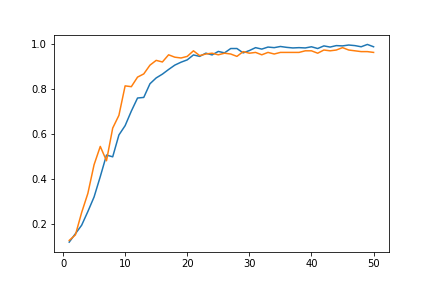
\includegraphics[width = \linewidth]{analysis/batch_size/b=1/b=1.png}
                    \captionof{figure}{Batch Size 1}
                \end{minipage}
                \hfill
                \begin{minipage}[b]{0.3\linewidth}
                    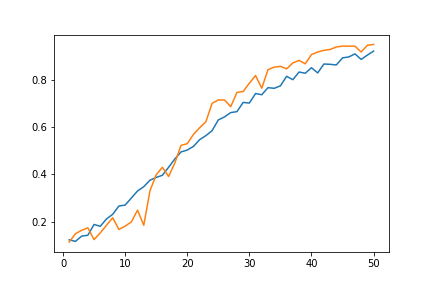
\includegraphics[width = \linewidth]{analysis/batch_size/b=5/b=5.png}
                    \captionof{figure}{Batch Size 5}
                \end{minipage}
                \hfill
                \begin{minipage}[b]{0.3\linewidth}
                    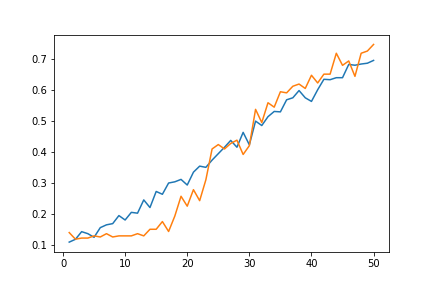
\includegraphics[width = \linewidth]{analysis/batch_size/b=10/b=10.png}
                    \captionof{figure}{Batch Size 10}
                \end{minipage}
            \end{center}
            A batch size of 1 leads to better and faster convergence.
        \item Batch Normalization
            \begin{center}
                \begin{minipage}[b]{0.45\linewidth}
                    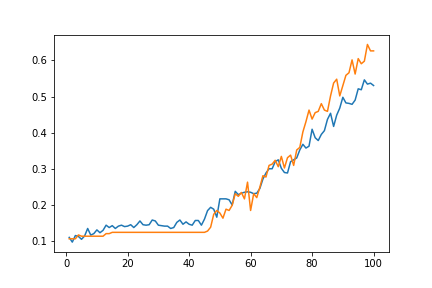
\includegraphics[width = \linewidth]{analysis/batchnorm/without/without.png}
                    \captionof{figure}{Without Batch Norm}
                \end{minipage}
                \hfill
                \begin{minipage}[b]{0.45\linewidth}
                    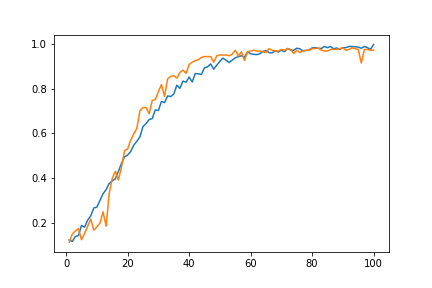
\includegraphics[width = \linewidth]{analysis/batchnorm/with/withbatchnorm.png}
                    \captionof{figure}{With Batch Norm}
                \end{minipage}
            \end{center}
            Faster convergence is observed with batch normalization.
            \item Optimizer
            \begin{center}
                \begin{minipage}[b]{0.45\linewidth}
                    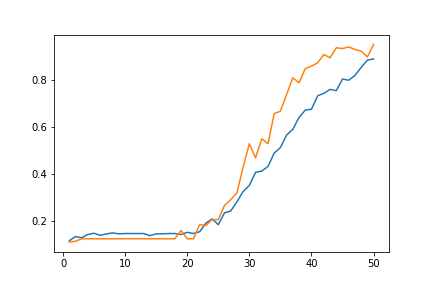
\includegraphics[width = \linewidth]{analysis/optimizer/adam/adam.png}
                    \captionof{figure}{Adam}
                \end{minipage}
                \hfill
                \begin{minipage}[b]{0.45\linewidth}
                    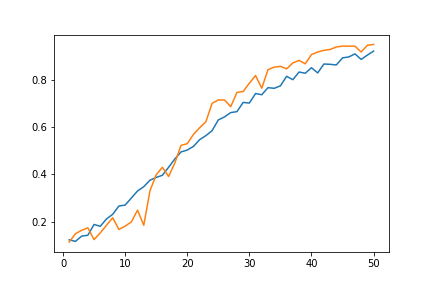
\includegraphics[width = \linewidth]{analysis/optimizer/sgd/sgd.png}
                    \captionof{figure}{SGD}
                \end{minipage}
            \end{center}
    \end{itemize}

    \bibliographystyle{abbrv}
    \bibliography{biblio}

\end{sloppypar}
\end{document}